%
%\begin{figure}
%\centering
%\begin{tabular}{cc}
%  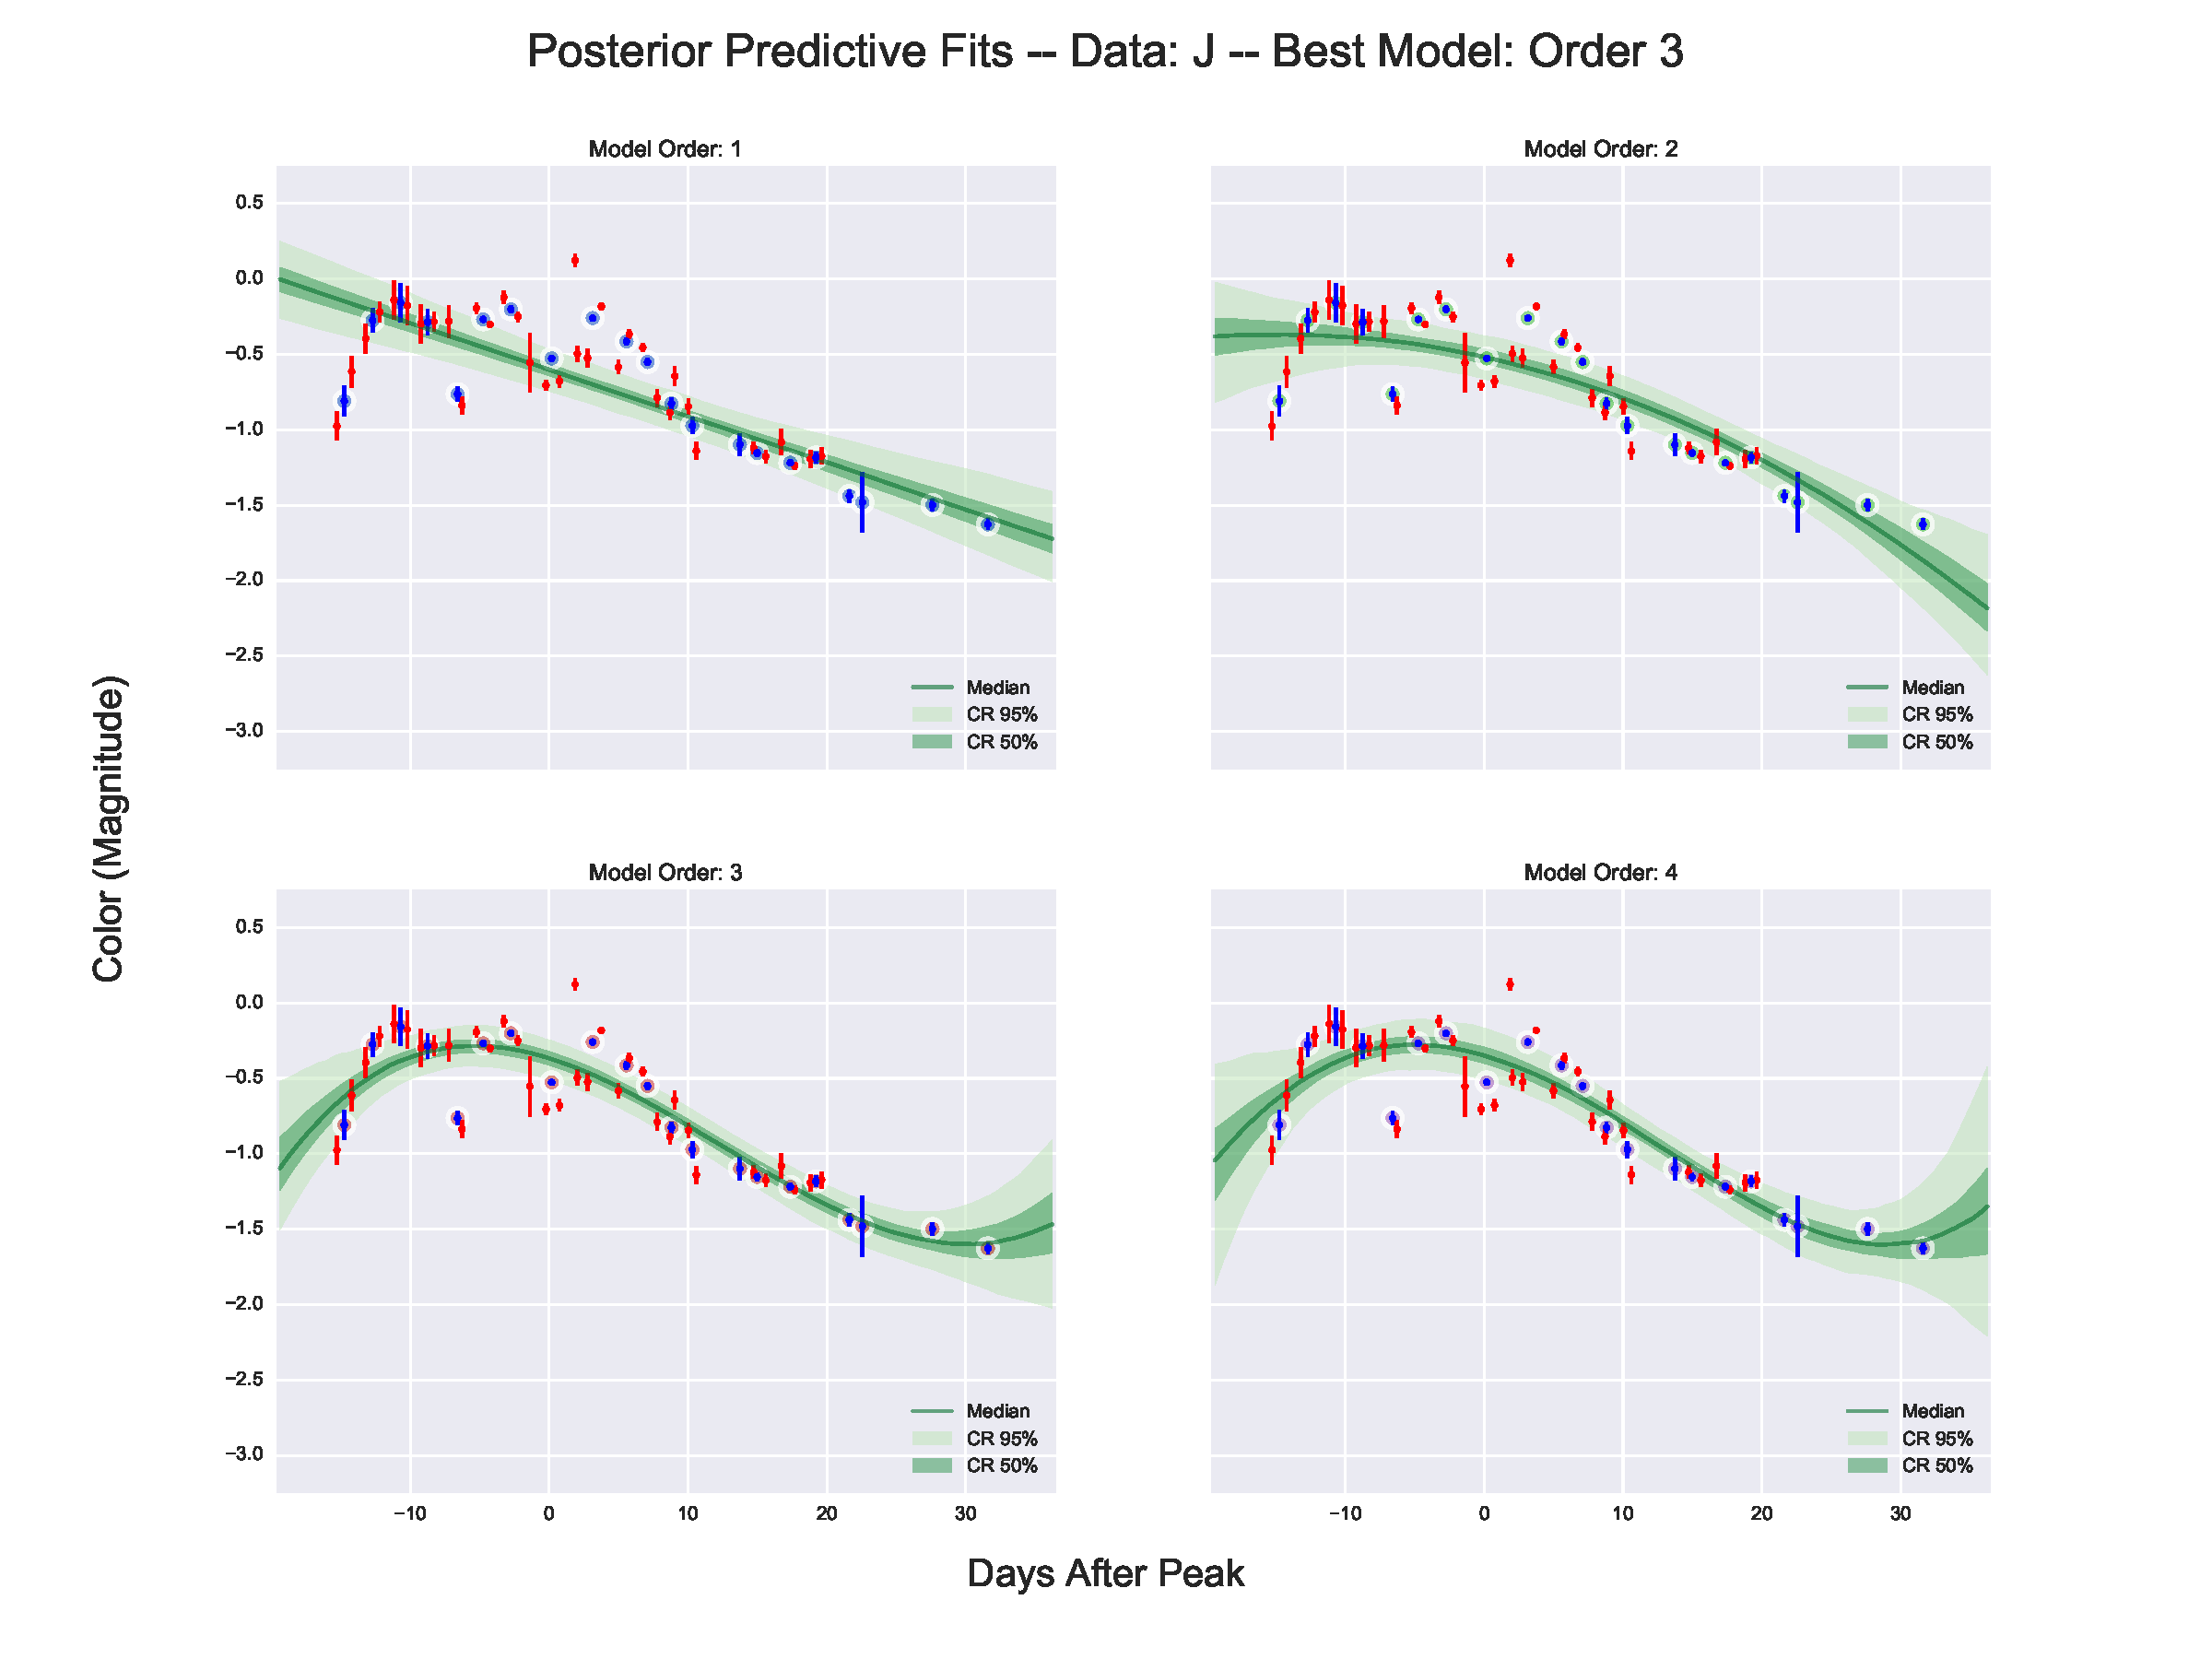
\includegraphics[scale=.35]{FIG/typeIb/J_fits} &   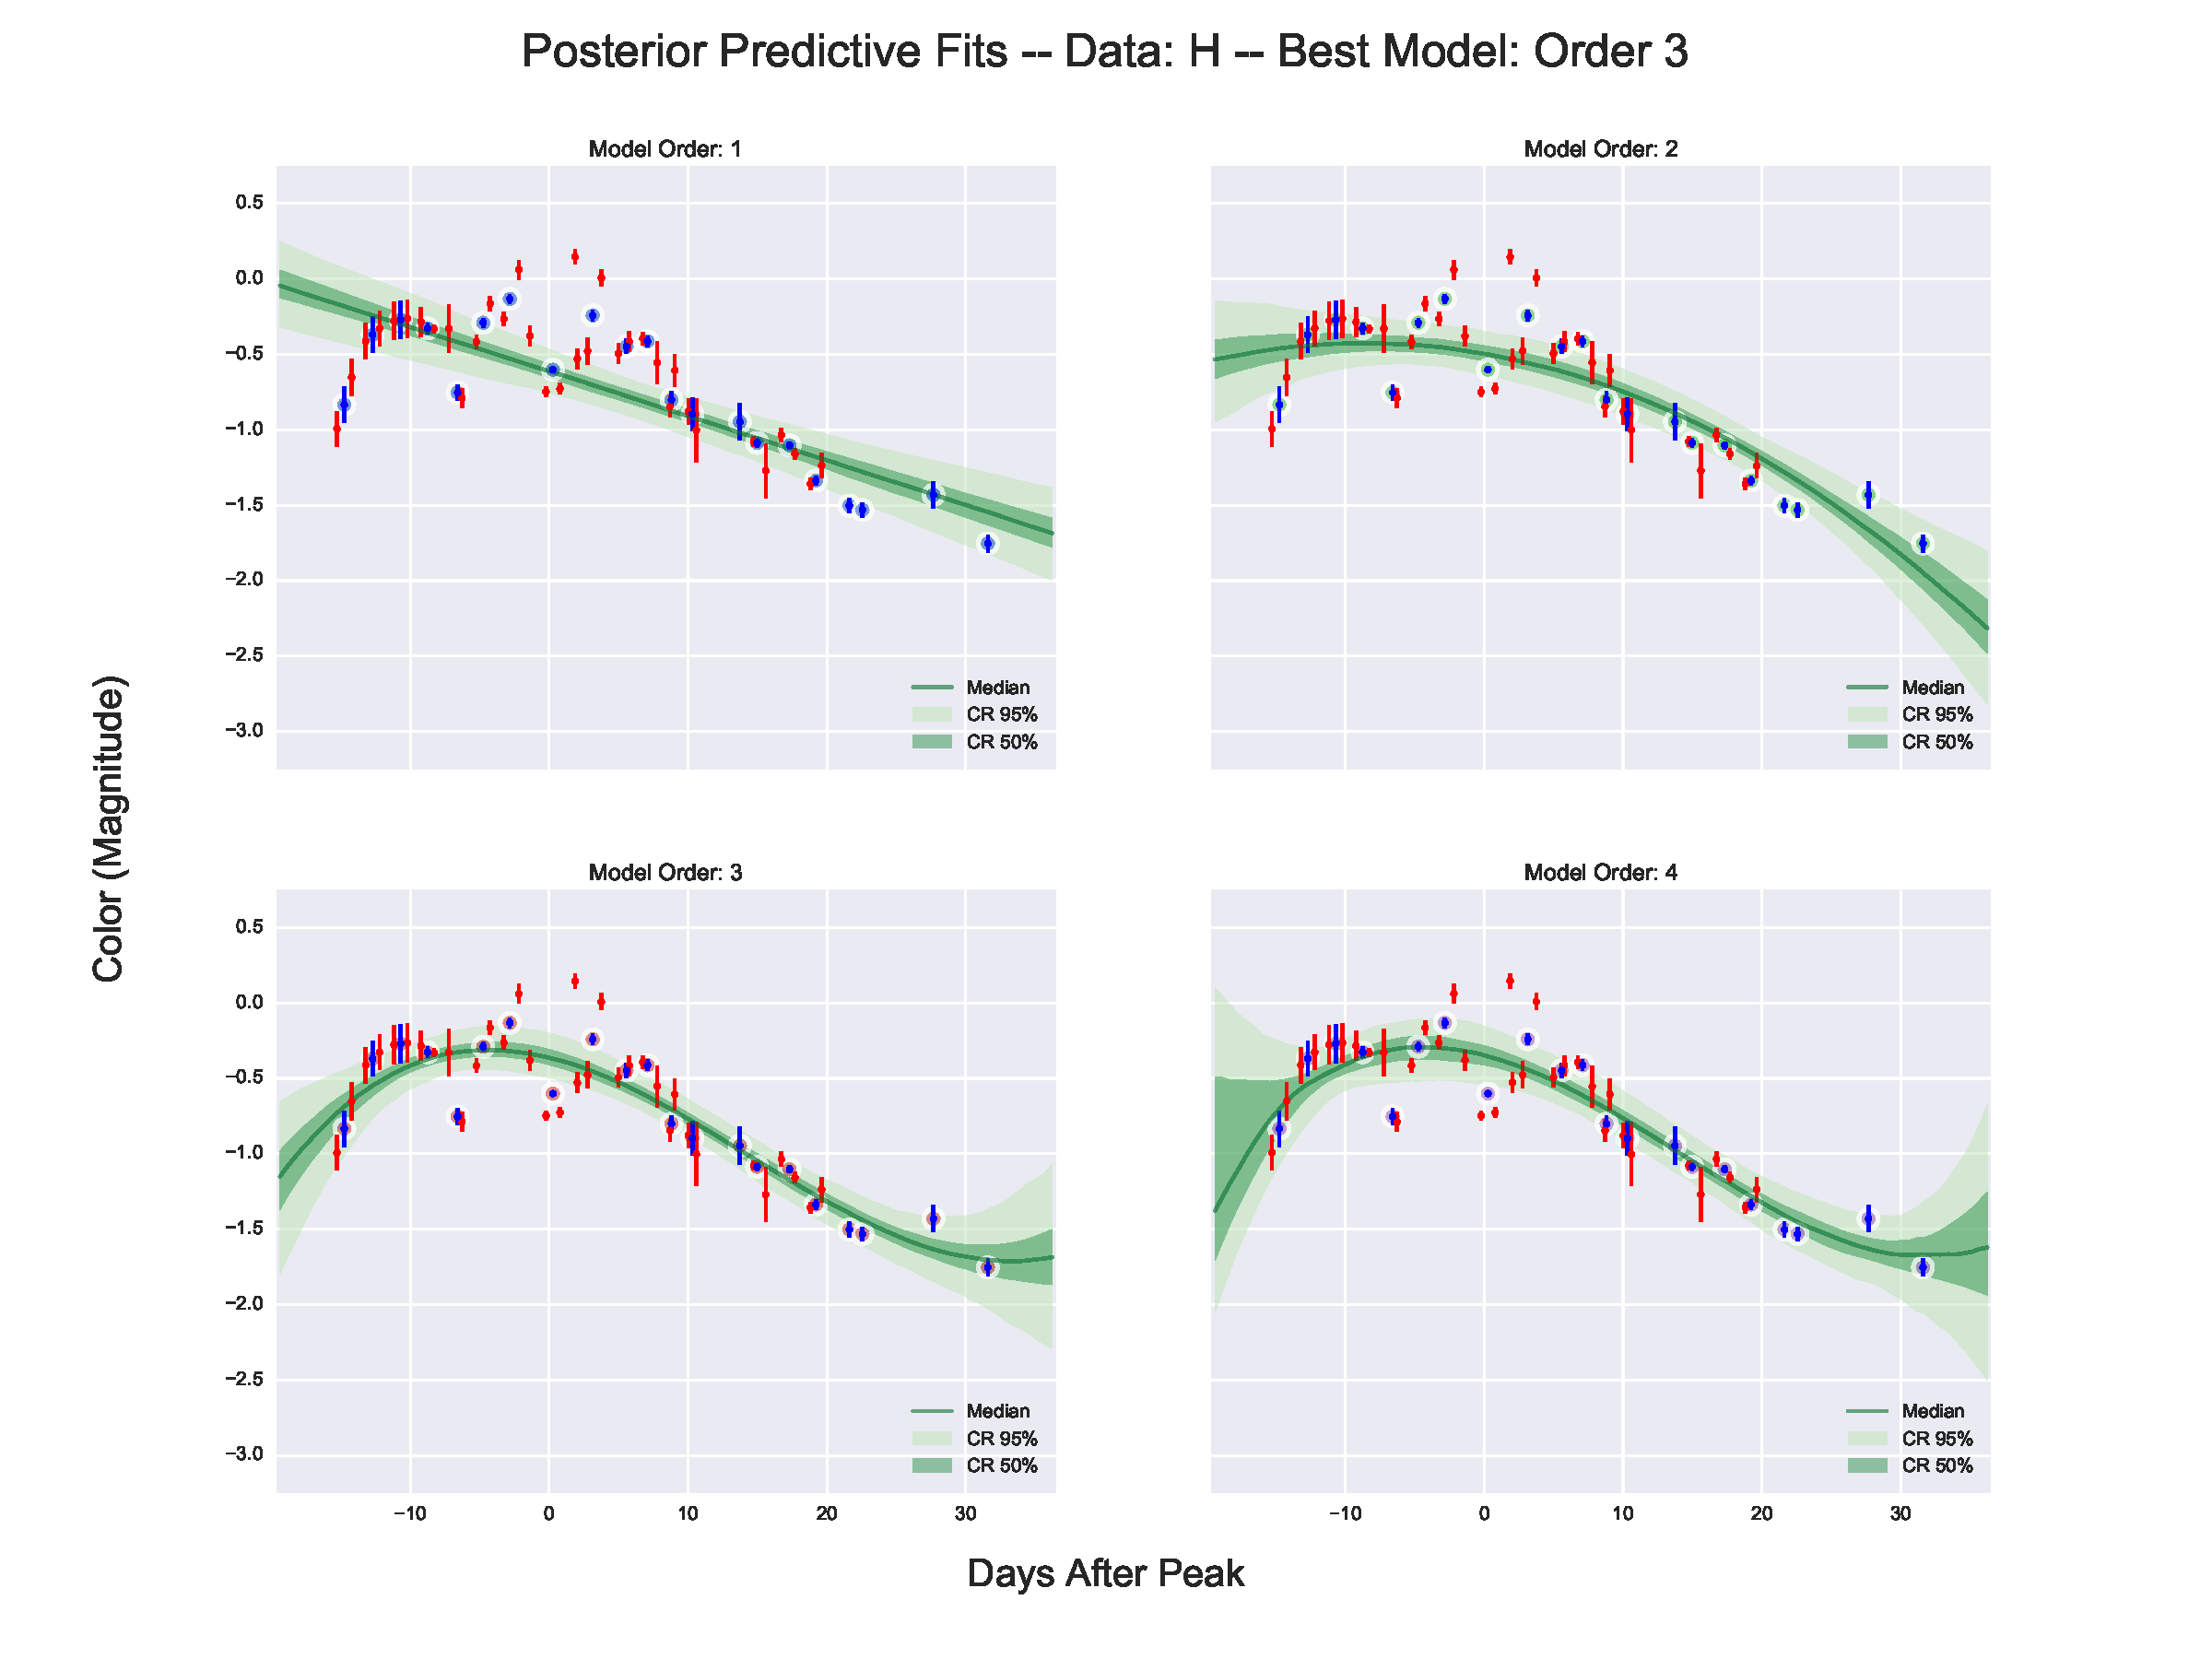
\includegraphics[scale=.35]{FIG/typeIb/H_fits} \\
%(a) first & (b) second \\[12pt]
% 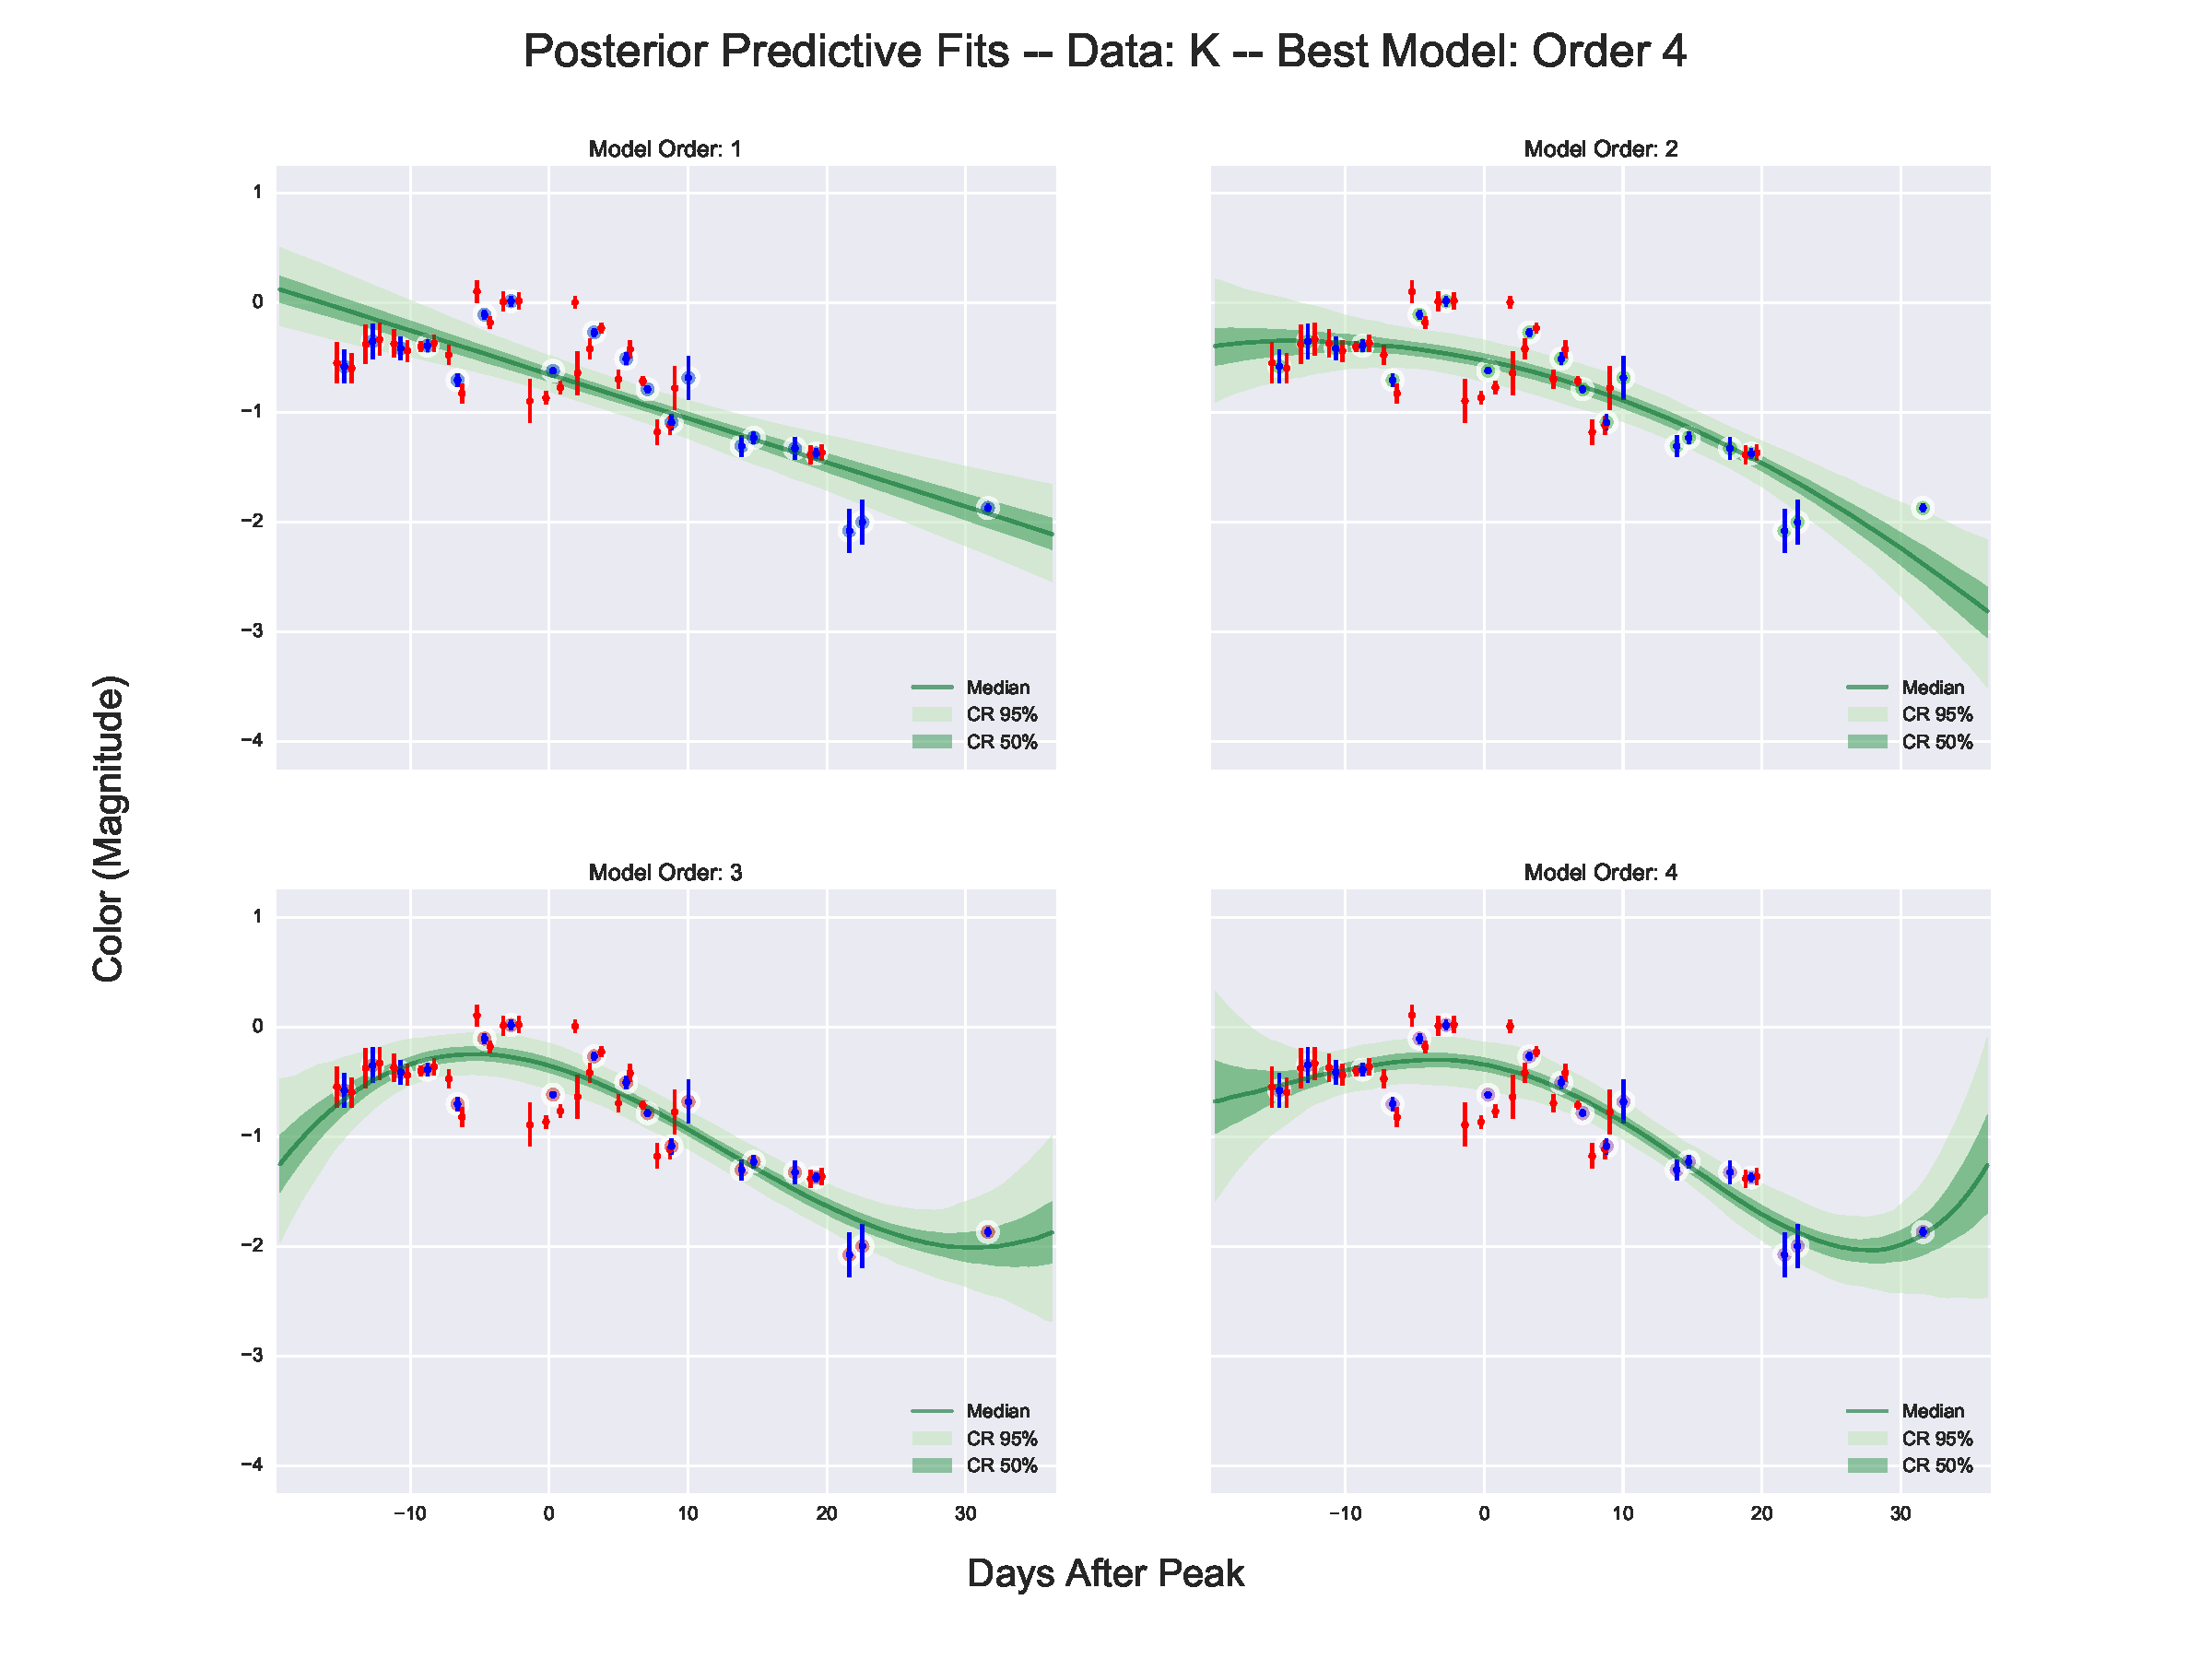
\includegraphics[scale=.35]{FIG/typeIb/K_fits} &   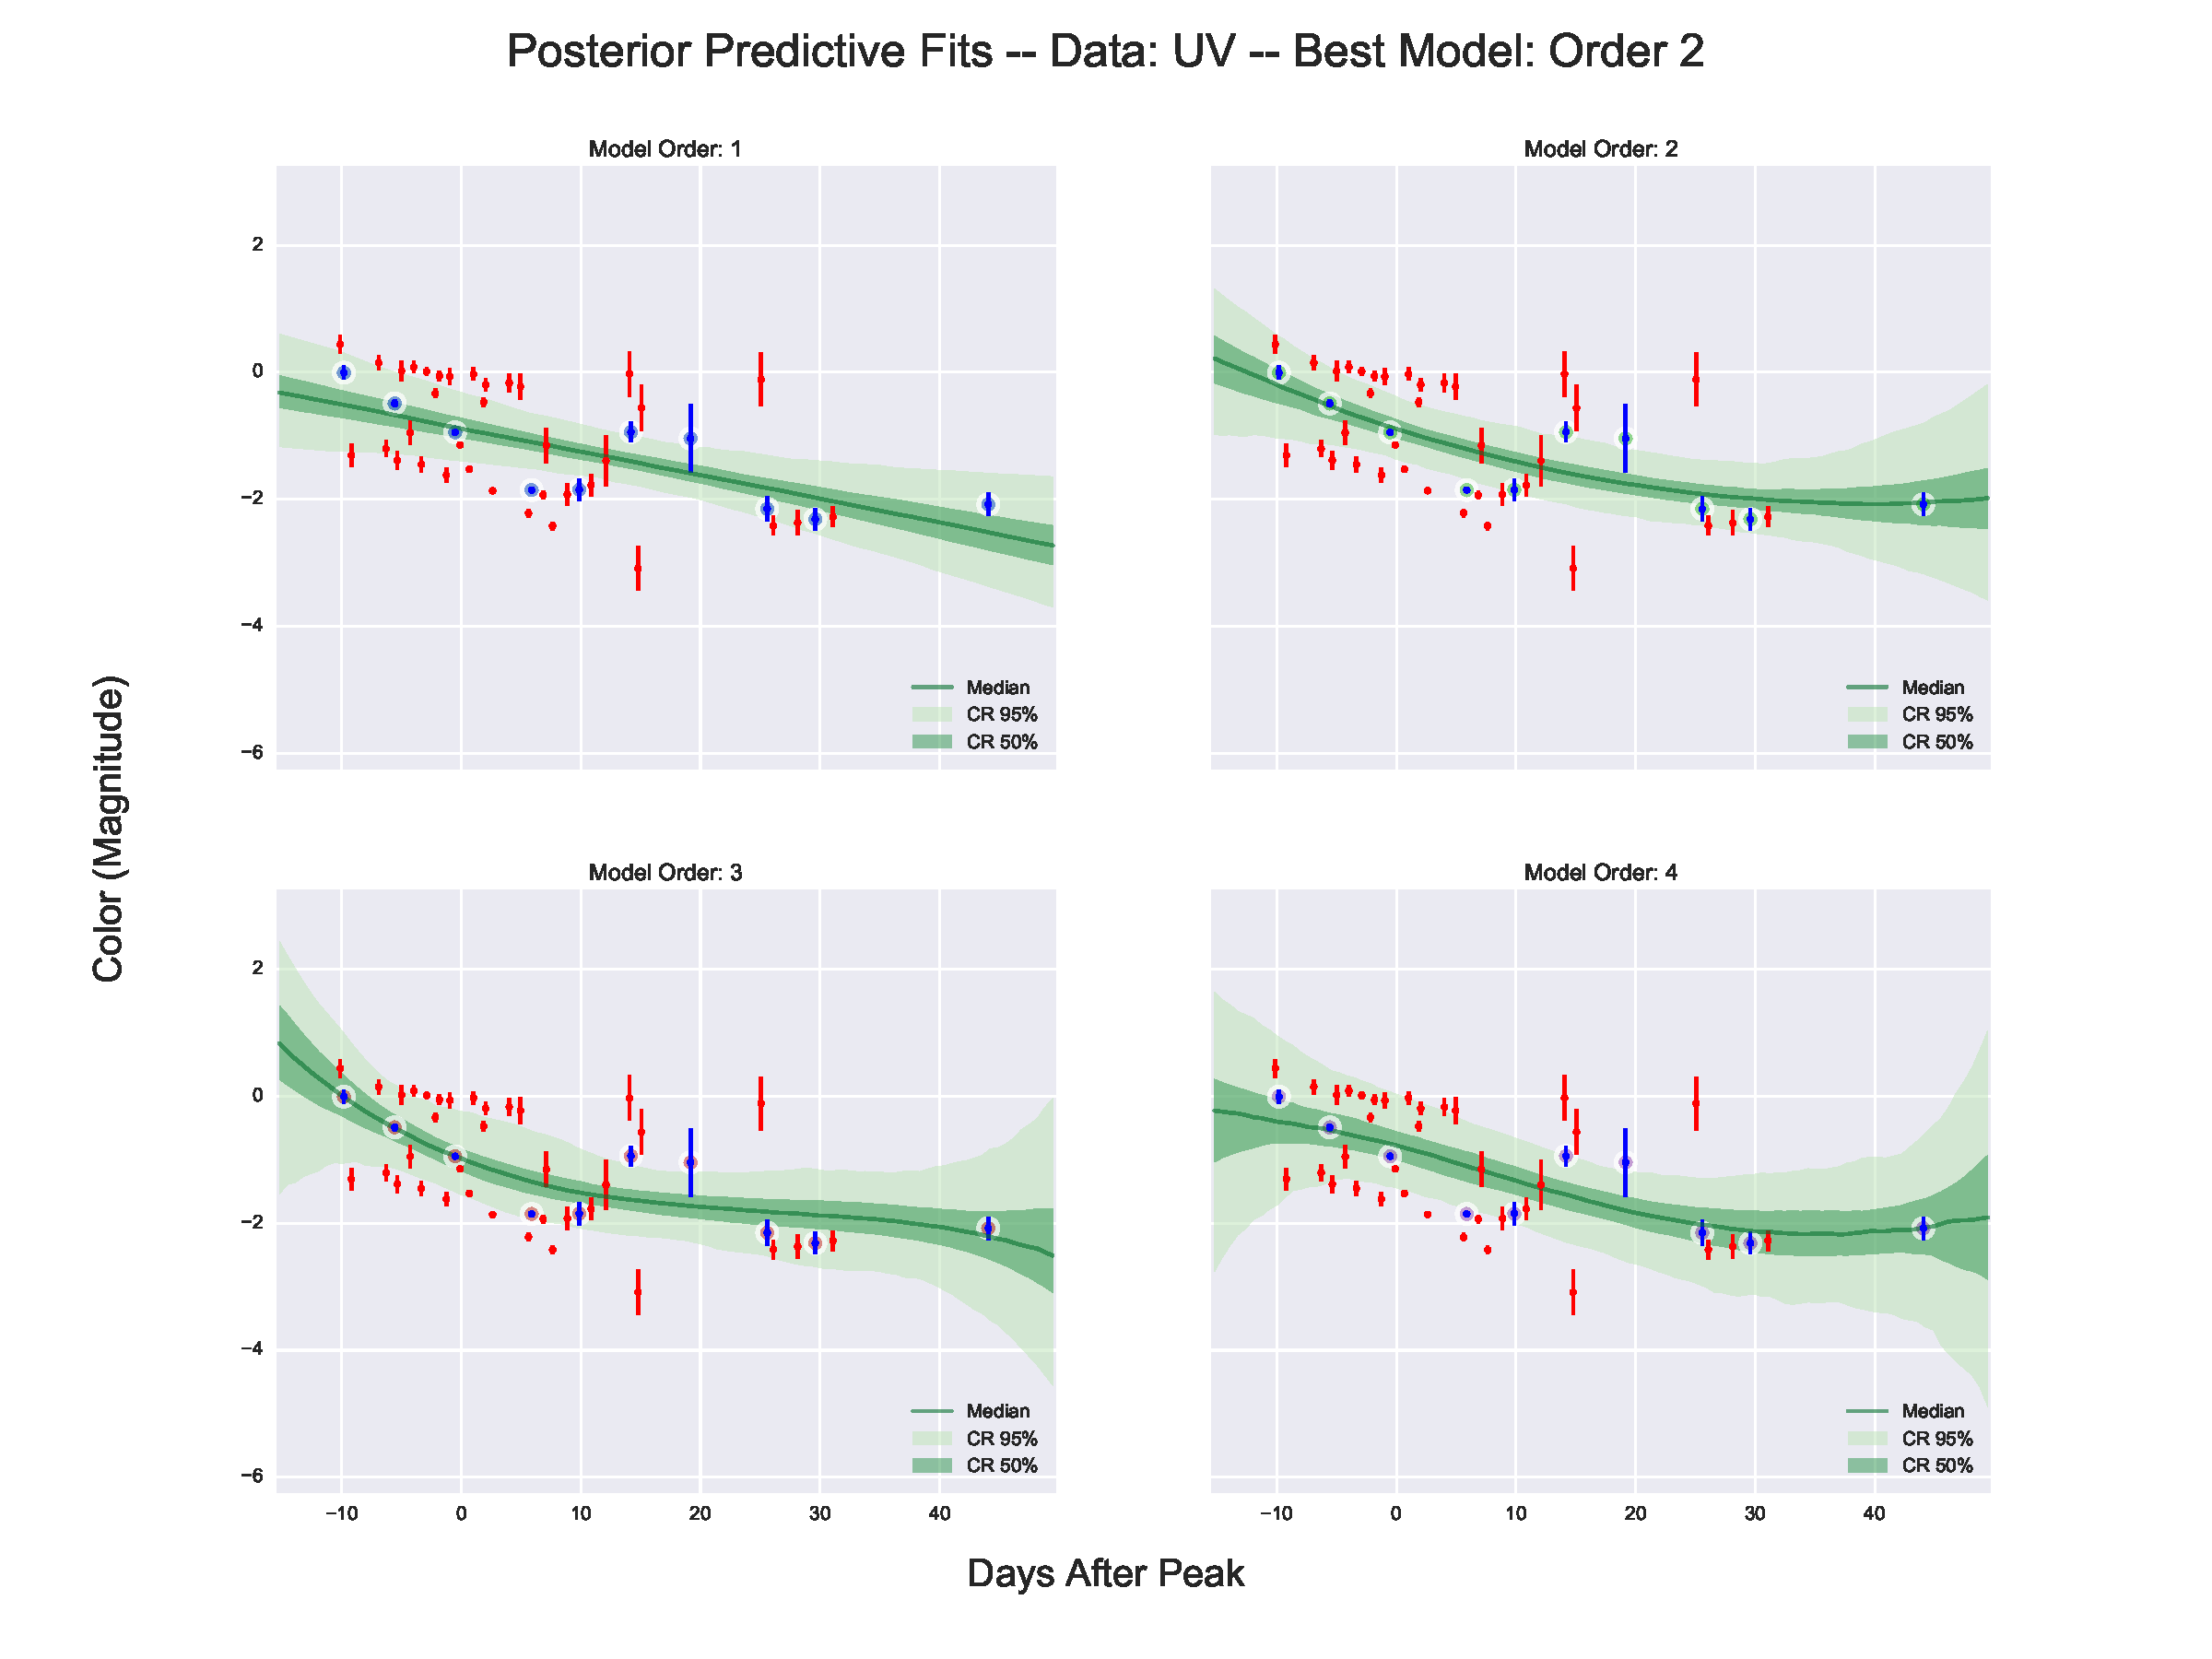
\includegraphics[scale=.35]{FIG/typeIb/UV_fits} \\
%(c) third & (d) fourth \\[12pt]
%\end{tabular}
%\caption{caption}
%\end{figure}
\subsection{Supernova Fitting}
\begin{figure}[H]
\centering
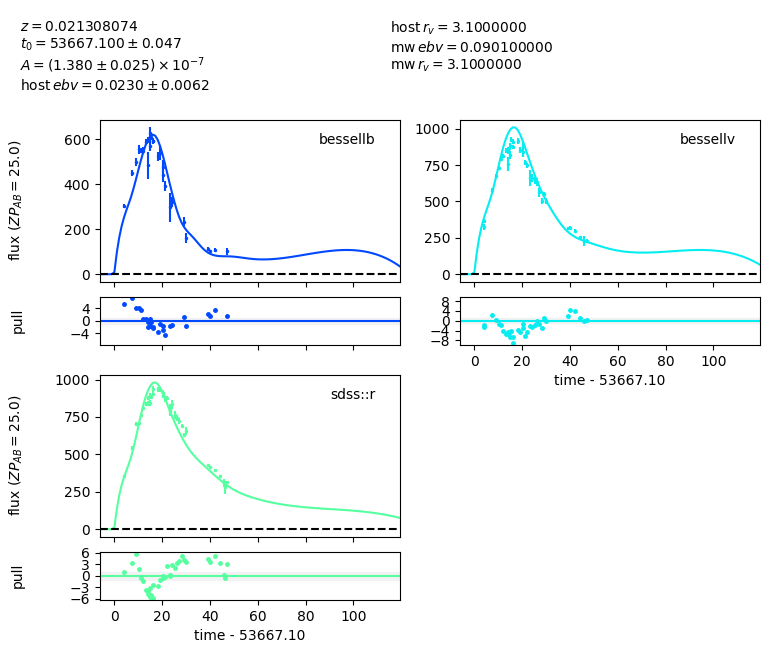
\includegraphics[scale=.75,center]{FIG/fits/lc_2005hg}
\caption{\label{fig:FIG/typeIb/J_fits} Example SNCOSMO fitting results of optical colors (B,V,r') for a SN Type Ib (SN 2005hg, see Table 1). For all SN fits see the appendix (I'll add them after tweaking).}
\end{figure}

\

\subsection{Color Curve Fitting}
\newcommand{\type}{II}
\begin{figure}[H]
\centering
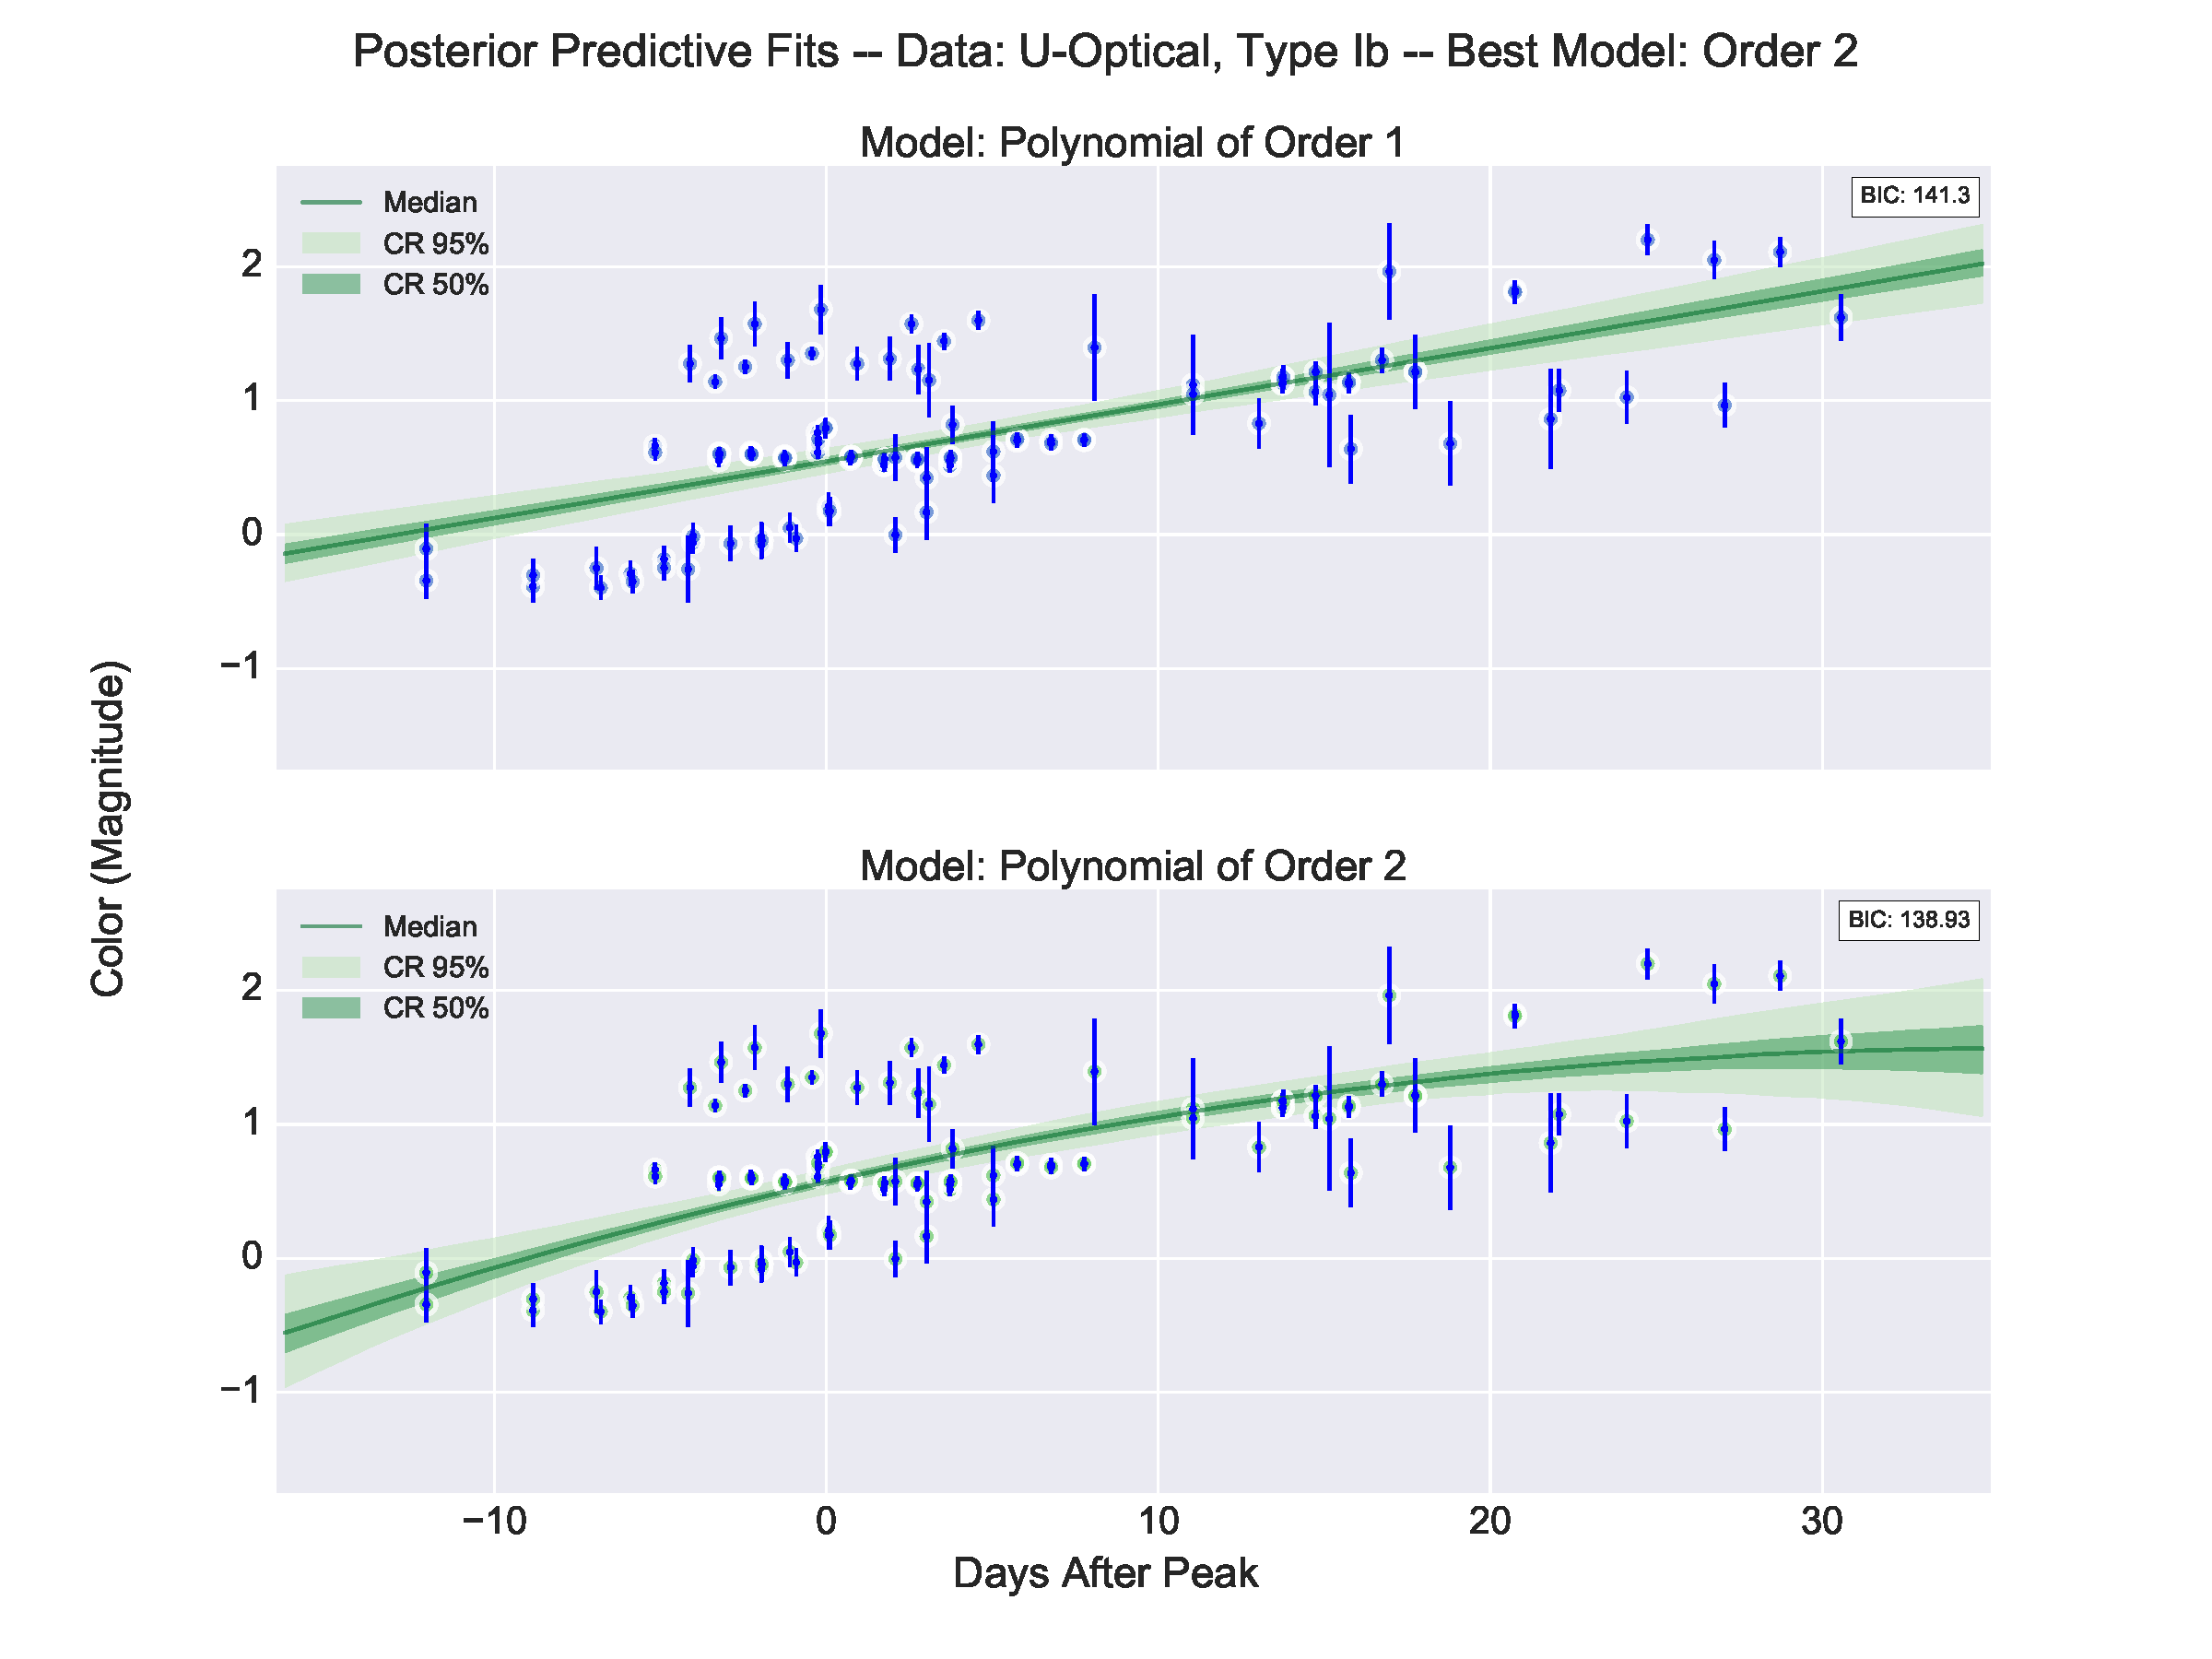
\includegraphics[scale=.5,center]{FIG/type\type/UV_fits}
\caption{\label{fig:FIG/typeIb/J_fits} Example Posterior Predictive fitting results for U-Optical colors measured from Type \type and Type IIP templates. The blue points represent binned data, while the red points represent the whole of the dataset (see section 3). The best fit model was chosen by minimizing the Bayesian Information Criterion. All fits to Optical-J,H,K for all SN types are shown in the appendix.}
\end{figure}

\subsection{SED Extrapolation}
\begin{figure}[H]
\centering
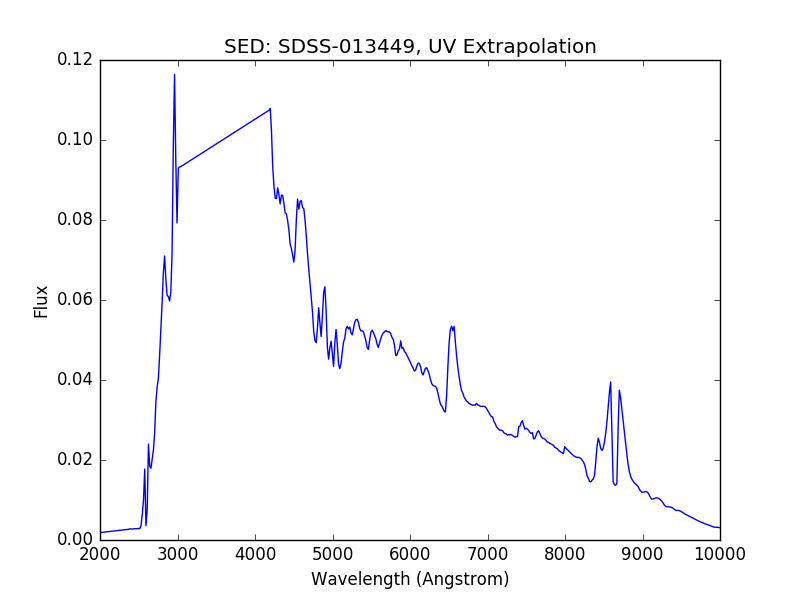
\includegraphics[scale=.75,center]{FIG/seds/SED}
\caption{\label{fig:FIG/typeIb/J_fits} Example of extrapolated SED into the UV using the color curve generated by the snsedextend package (This was just an example, I'll run all of them once we decide all of the tweaks, etc.)}
\end{figure}
\bigskip
